% SPIE Defense + Security 2026 — Poster 14030-26
% 36" x 42" (SPIE standard), sans-serif, readable from 3-6 feet
%
\documentclass[25pt, blockverticalspace=5mm, colspace=12mm, margin=0.75in]{tikzposter}

% --- Override paper dimensions to SPIE 36in x 42in ---
% geometry (loaded by tikzposter) defaults to a0paper.  Override it here
% so its \AtBeginDocument hook sets \textwidth/\textheight correctly.
% tikzposter then derives \TP@visibletextwidth/height on top of those.
\geometry{paperwidth=36in, paperheight=42in, margin=0.75in}
\makeatletter
\setlength{\TP@visibletextwidth}{\dimexpr 36in - 1.5in\relax}
\setlength{\TP@visibletextheight}{\dimexpr 42in - 1.5in\relax}
\pdfpagewidth=36in
\pdfpageheight=42in
\makeatother

% --- Remove tikzposter watermark ---
\tikzposterlatexaffectionproofoff

% --- Fonts (sans-serif per SPIE guidelines) ---
\usepackage[T1]{fontenc}
\usepackage{helvet}
\renewcommand{\familydefault}{\sfdefault}

% --- Math ---
\usepackage{amsmath}
\usepackage{amssymb}

% --- Graphics ---
\usepackage{graphicx}
\graphicspath{{figures/}}

% --- Tables ---
\usepackage{booktabs}
\usepackage{array}

% --- Units ---
\usepackage{siunitx}
\sisetup{per-mode=symbol}

% --- Compact lists ---
\usepackage{enumitem}
\setlist{nosep, leftmargin=1.5em}

% --- Color theme ---
\definecolor{spieblue}{HTML}{1A5276}
\definecolor{spieltblue}{HTML}{E8F0FE}
\definecolor{spieaccent}{HTML}{CC5500}
\definecolor{spiebg}{HTML}{FFFFFF}

% --- tikzposter theme ---
\usetheme{Default}
\definecolorstyle{SPIEStyle}{
    \definecolor{colorOne}{named}{spieblue}
    \definecolor{colorTwo}{named}{spieltblue}
    \definecolor{colorThree}{named}{spieaccent}
}{
    \colorlet{backgroundcolor}{spiebg}
    \colorlet{framecolor}{colorOne}
    \colorlet{titlefgcolor}{white}
    \colorlet{titlebgcolor}{colorOne}
    \colorlet{blocktitlebgcolor}{colorOne}
    \colorlet{blocktitlefgcolor}{white}
    \colorlet{blockbodybgcolor}{white}
    \colorlet{blockbodyfgcolor}{black}
    \colorlet{innerblocktitlebgcolor}{colorTwo}
    \colorlet{innerblocktitlefgcolor}{colorOne}
    \colorlet{innerblockbodybgcolor}{white}
    \colorlet{innerblockbodyfgcolor}{black}
}
\usecolorstyle{SPIEStyle}
\useblockstyle{Default}

% Use Filled title style (single dark banner)
\usetitlestyle{Filled}

% --- Fix tikzposter duplicate-title bug ---
% tikzposter's \maketitle renders a "transparent" dummy node that is actually
% visible (not a valid TikZ key). Replace with savebox measurement.
\makeatletter
\newsavebox{\TP@titlebox}
\renewcommand\maketitle[1][]{%
    \normalsize
    \setkeys{title}{#1}%
    % Measure title height without rendering
    \sbox{\TP@titlebox}{\parbox{\TP@titlewidth-2\TP@titleinnersep}{\TP@maketitle}}%
    \setlength{\TP@titleheight}{\dimexpr\ht\TP@titlebox+\dp\TP@titlebox+2\TP@titleinnersep+6em\relax}%
    \global\TP@titleheight=\TP@titleheight
    \setlength{\titleheight}{\TP@titleheight}%
    \global\titleheight=\titleheight
    % Compute title position
    \setlength{\titleposleft}{-0.5\titlewidth}%
    \setlength{\titleposright}{\titleposleft+\titlewidth}%
    \setlength{\titlepostop}{0.5\textheight-\TP@titletotopverticalspace}%
    \setlength{\titleposbottom}{\titlepostop-\titleheight}%
    % Title background
    \TP@titlestyle
    % Title text — single node, no dummy
    \node[inner sep=\TP@titleinnersep, line width=\TP@titlelinewidth,
          anchor=north, minimum width=\TP@visibletextwidth-2\TP@titleinnersep]
        at (0,0.5\textheight-\TP@titletotopverticalspace)
        {\parbox{\TP@titlewidth-2\TP@titleinnersep}{\TP@maketitle}};%
    \normalsize
    \setlength{\TP@blocktop}{\titleposbottom-\TP@titletoblockverticalspace}%
}
\makeatother

% --- Override TP@maketitle to remove \sc (small caps) from title ---
\makeatletter
\gdef\TP@maketitle{%
    \centering
    \vbox{%
        \@titlegraphic\\[\TP@titlegraphictotitledistance]%
        \centering
        \color{titlefgcolor}%
        {\bfseries \Huge \@title \par}%
        \vspace*{0.7em}%
        {\huge \@author \par}%
        \vspace*{0.7em}%
        {\LARGE \@institute}%
    }%
}
\makeatother

% ============================================================================
\title{\parbox{0.95\linewidth}{\centering
    Predictive Target Pursuit for Autonomous UAVs using RF-DETR \\[2mm]
    with Depth-Aware State Estimation and Physics-Informed Trajectory Prediction
}}

\author{%
    \textbf{Rylan Malarchick}\textsuperscript{*},
    Carmen DiMario,
    Enrique Amaya,
    Graysen Brinkman,
    Sajid Berhane,
    and Jose Castelblanco%
}

\institute{%
    Engineering Physics Propulsion Lab (EPPL), Embry-Riddle Aeronautical University, Daytona Beach, FL \\[2mm]
    {\textsuperscript{*}malarchr@my.erau.edu} \quad\textbar\quad
    {SPIE Defense + Security 2026} \quad\textbar\quad
    {Paper 14030-26}\\[1mm]
    {DS112: Machine Learning from Challenging Data}%
}

% ============================================================================
\begin{document}

\maketitle

\begin{columns}

% ============================== COLUMN 1 ==============================
\column{0.33}

% --- Motivation ---
\block{Motivation}{
    Autonomous UAV pursuit of airborne targets faces two compounding challenges:

    \begin{itemize}
        \item \textbf{Detection degrades} under adverse visual conditions (noise, low light, motion blur, occlusion)
        \item \textbf{Reactive controllers fail} when detections disappear --- no input means the pursuer drifts off target
    \end{itemize}

    \vspace{2mm}
    \textbf{AIRHOUND} addresses both within a single onboard system: a \textbf{robust transformer detector} (RF-DETR) paired with \textbf{physics-informed prediction} (PINN) that maintains tracking through multi-second dropouts.

    \vspace{2mm}
    \coloredbox[bgcolor=spieltblue,fgcolor=spieblue]{
        \textbf{Key question:} Can architecture choice improve detection robustness under degraded conditions, and can learned prediction bridge the remaining dropout gaps?
    }
}

% --- System Architecture ---
\block{System Architecture}{
    \begin{tikzfigure}[AIRHOUND perception-to-control pipeline on the Jetson Orin. All nodes communicate via ROS\,2 topics over Micro XRCE-DDS to the PX4 flight controller.]
        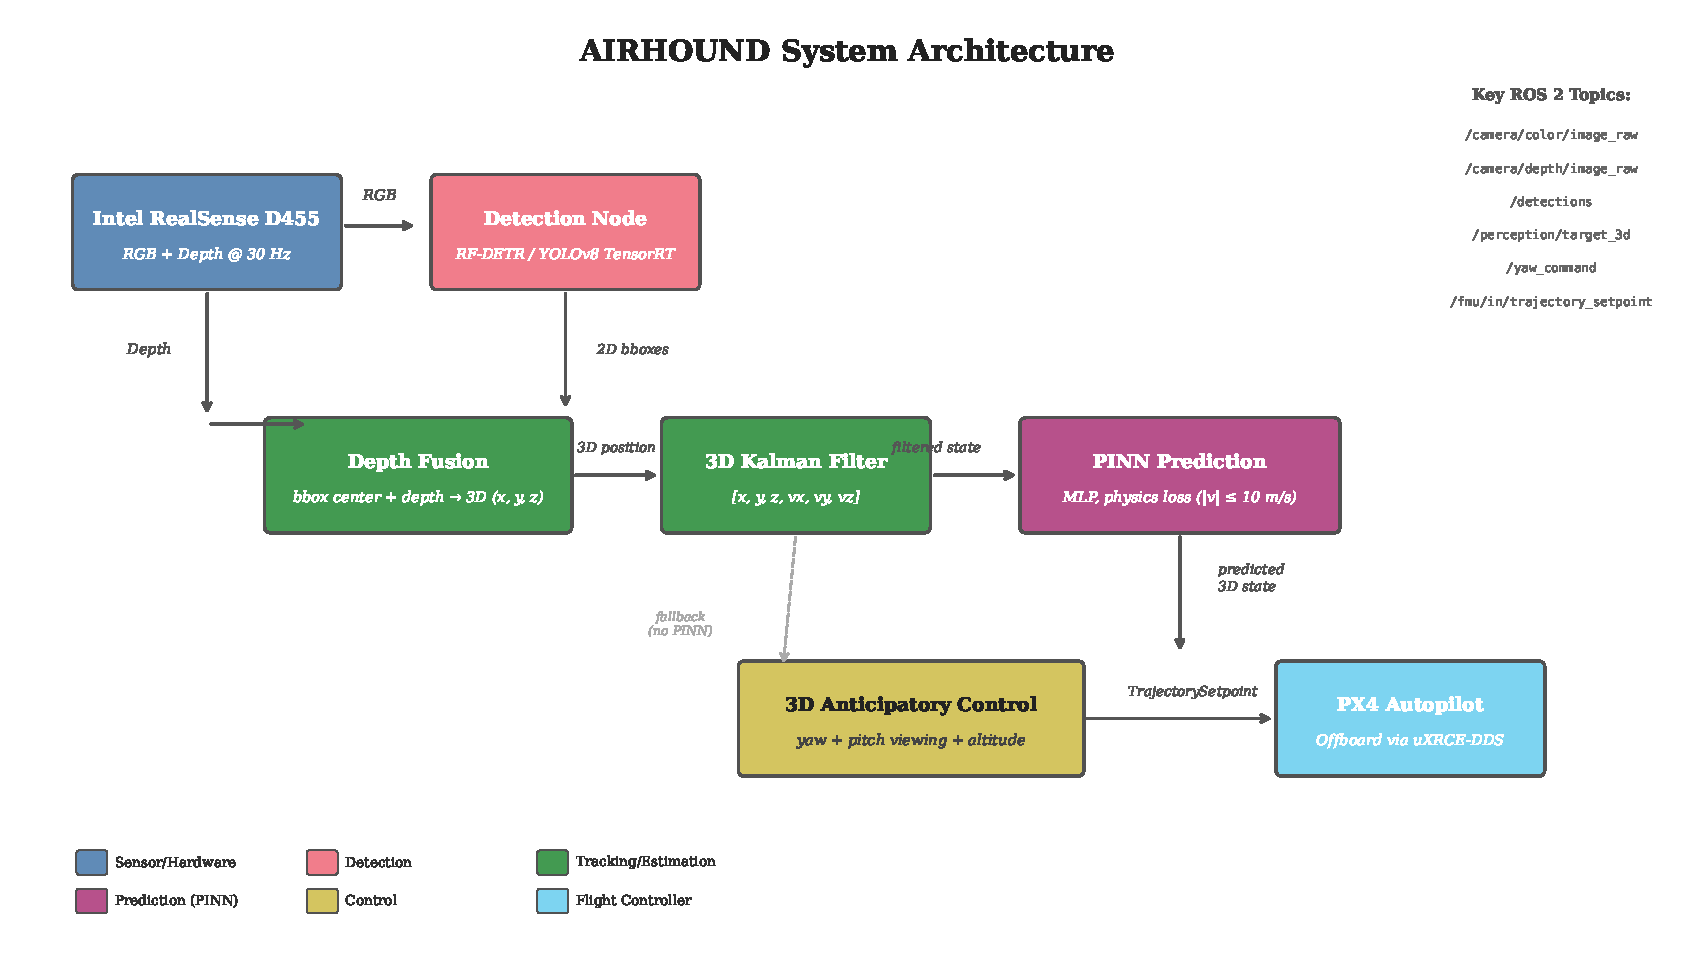
\includegraphics[width=0.90\linewidth]{system_architecture.pdf}
    \end{tikzfigure}

    \textbf{Hardware platform:}
    \begin{itemize}
        \item NVIDIA Jetson Orin Nano (16\,GB) --- all inference onboard
        \item Intel RealSense D455 stereo camera
        \item Auterion PX4 FMUv6X flight controller (HIL mode)
        \item ROS\,2 Humble with runtime YAML configuration
    \end{itemize}
}

% --- PINN ---
\block{Physics-Informed Trajectory Prediction}{
    During detection dropout, the PINN predicts target trajectory with a velocity-bounded physics loss:
    \[
        \mathcal{L} = \mathcal{L}_{\text{data}} + \lambda \cdot \max\!\bigl(0,\; \|\mathbf{v}\| - v_{\max}\bigr)^{2}
    \]

    \begin{itemize}
        \item Prevents physically implausible extrapolation $(v_{\max} = 10\,\text{m/s})$
        \item TensorRT FP16 engine: \textbf{0.28\,ms} inference on Jetson GPU
        \item Maintains tracking through dropouts up to \textbf{16.3\,s} in HITL testing
        \item 77.5\% of tracking time in PINN mode during synthetic dropout test
    \end{itemize}
}


% ============================== COLUMN 2 ==============================
\column{0.34}

% --- Degradation Robustness ---
\block{Degradation Robustness: RF-DETR vs.\ YOLOv8n}{
    Both detectors evaluated under 4 degradation types $\times$ 5 severity levels on 1,983 validation images (Roboflow Drones dataset).

    \begin{tikzfigure}[Detection accuracy (mAP@0.5) under increasing degradation severity. RF-DETR (transformer) maintains substantially higher accuracy than YOLOv8n (CNN) under Gaussian noise and low-light conditions.]
        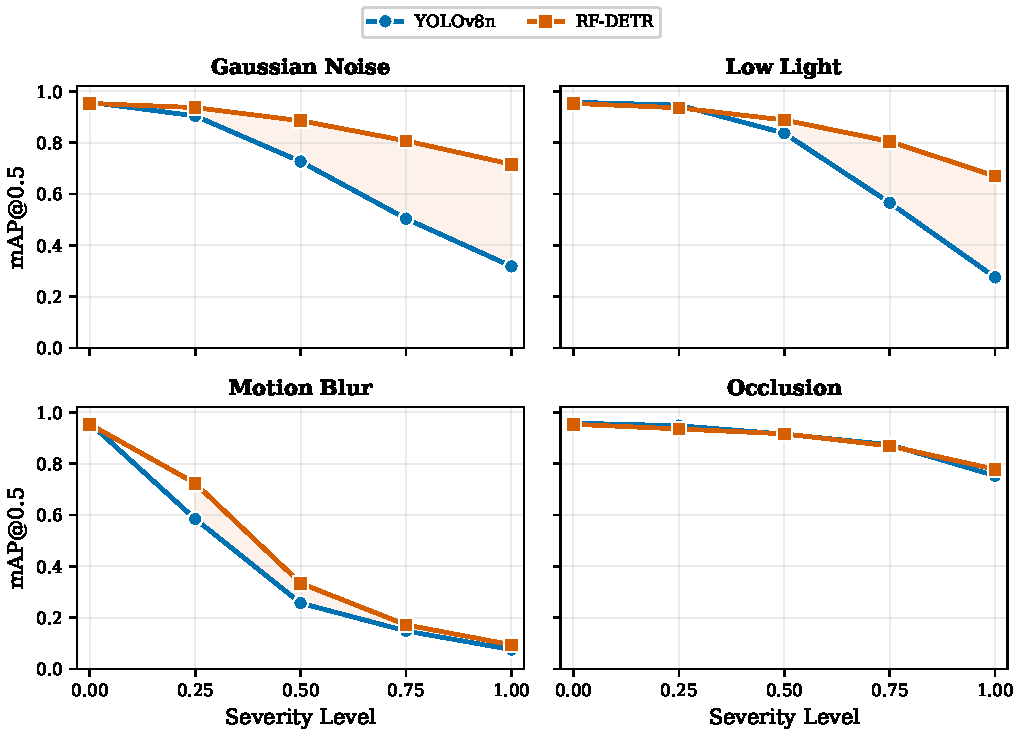
\includegraphics[width=0.95\linewidth]{degradation_comparison.pdf}
    \end{tikzfigure}

    \vspace{2mm}
    \coloredbox[bgcolor=spieltblue,fgcolor=spieblue]{
        \centering
        \textbf{At maximum noise severity:} RF-DETR achieves \textbf{0.716} mAP@0.5 \\ vs.\ YOLOv8n at \textbf{0.318} --- a \textbf{+39.8\,pp} advantage
    }

    \vspace{2mm}
    \begin{tikzfigure}[Percentage of clean-baseline mAP retained under increasing severity for Gaussian noise and low light --- the conditions with the largest architectural gap.]
        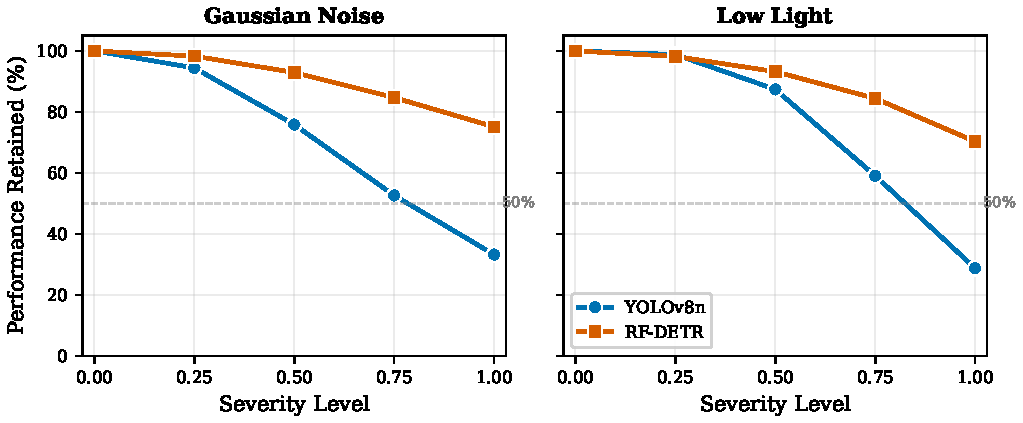
\includegraphics[width=0.95\linewidth]{retention_curve.pdf}
    \end{tikzfigure}

    \vspace{2mm}
    \textbf{Why transformers win:} Self-attention aggregates global context --- uncorrupted image regions still contribute to detection even when local patches are degraded. CNN local receptive fields lose access to clean features proportionally to corruption.
}

% --- References ---
\block{References}{
    \small
    \begin{enumerate}[label={[\arabic*]}, nosep, leftmargin=2em]
        \item Y.~Zhao et al., ``Real-Time Detection Transformer,'' \textit{Proc.\ IEEE/CVF CVPR}, 2024.
        \item G.~Jocher, A.~Chaurasia, and J.~Qiu, ``Ultralytics YOLOv8,'' 2023.
        \item M.~Raissi, P.~Perdikaris, and G.~E.~Karniadakis, ``Physics-informed neural networks,'' \textit{J.~Comput.\ Phys.}, vol.~378, pp.~686--707, 2019.
        \item L.~Meier, D.~Honegger, and M.~Pollefeys, ``PX4: A node-based multithreaded open source robotics framework,'' \textit{Proc.\ IEEE ICRA}, 2015.
        \item Roboflow, ``Drone Detection Dataset,'' 2023.
    \end{enumerate}
}


% ============================== COLUMN 3 ==============================
\column{0.33}

% --- HITL Validation ---
\block{Hardware-in-the-Loop Validation}{
    End-to-end pipeline tested with PX4 FMUv6X in HIL mode. Six configurations spanning synthetic and camera inputs.

    \begin{center}
    \small
    \renewcommand{\arraystretch}{1.15}
    \begin{tabular}{l r r r r}
        \toprule
        \textbf{Config} & \textbf{Det.\,Rate} & \textbf{Latency} & \textbf{P95} & \textbf{Dropouts} \\
         & (\%) & (ms) & (ms) & \\
        \midrule
        \multicolumn{5}{l}{\textit{Synthetic (mock detector, simulated dropouts)}} \\
        Sim\,A & 22.9 & --- & --- & 4 \\
        Sim\,B & 21.9 & --- & --- & 10 \\
        Sim\,C\textsuperscript{$\dagger$} & 21.0 & --- & --- & 16 \\
        \midrule
        \multicolumn{5}{l}{\textit{Camera (RF-DETR TensorRT, RealSense D455)}} \\
        Cam\,640 (bridge) & 100.0 & 234.5 & 598.1 & 1 \\
        Cam\,720 (bridge) & 59.5 & 233.7 & 558.2 & 114 \\
        \midrule
        \textbf{Cam\,Direct} & \textbf{100.0} & \textbf{58.8} & \textbf{61.5} & \textbf{0} \\
        \bottomrule
        \multicolumn{5}{l}{\footnotesize\textsuperscript{$\dagger$}PINN fallback enabled; 77.5\% of tracking in PINN mode.}
    \end{tabular}
    \end{center}
}

% --- V4L2 Optimization ---
\block{V4L2 Direct Capture Optimization}{
    \begin{tikzfigure}[Mean and P95 inference latency by capture method. V4L2 direct capture eliminates the DDS serialization bottleneck, reducing latency 4$\times$.]
        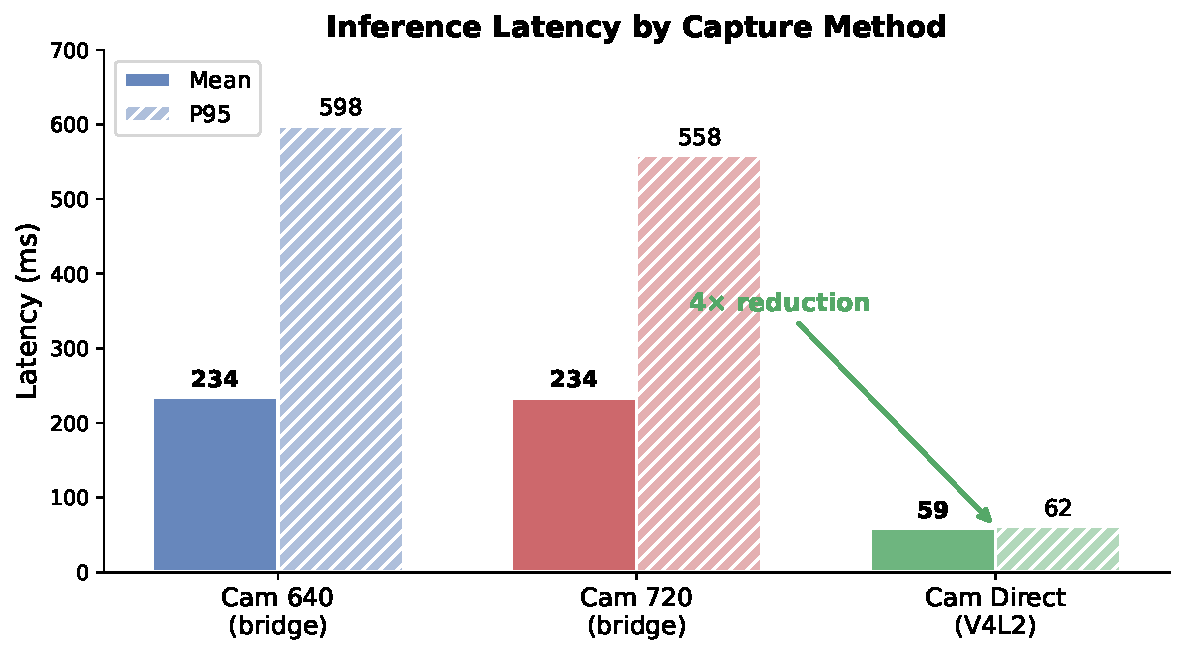
\includegraphics[width=0.95\linewidth]{latency_poster.pdf}
    \end{tikzfigure}

    ROS\,2 DDS cannot serialize 2.7\,MB BGR8 frames fast enough --- bridge caps at $\sim$1.5\,FPS in Python. \textbf{Integrating V4L2 capture directly into the detector node} bypasses DDS image transport:

    \begin{itemize}
        \item \textbf{4$\times$} latency reduction (234\,ms $\rightarrow$ 58.8\,ms mean)
        \item \textbf{10$\times$} lower latency variance (P95: 598\,ms $\rightarrow$ 61.5\,ms)
        \item \textbf{100\%} detection rate at 1280$\times$720 (was 59.5\% via bridge)
        \item \textbf{Zero} dropouts over 108-second test
    \end{itemize}
}

% --- Conclusions ---
\block{Conclusions}{
    \begin{enumerate}
        \item \textbf{RF-DETR} retains 75\% clean mAP at max noise severity vs.\ 33\% for YOLOv8n (+39.8\,pp advantage)
        \item \textbf{PINN prediction} maintains tracking through 16.3\,s dropouts with velocity-bounded extrapolation
        \item \textbf{Direct V4L2 capture} achieves 58.8\,ms inference at 15\,FPS --- real-time on edge hardware
        \item \textbf{Modular ROS\,2 pipeline} enables runtime component selection via single YAML config
    \end{enumerate}

    \smallskip
    \textbf{Future work:} Free-flight validation, multi-axis control, PINN retraining on real trajectories.

    \vspace{5mm}
    \hrule
    \vspace{4mm}
    {\footnotesize\textit{Acknowledgments:} Conducted at EPPL, Embry-Riddle Aeronautical University, under Dr.\ Sergey Drakunov. Supported by SPIE Student Conference Support grant, and ERAU UGR Spark grant.}
}

\end{columns}

\end{document}
